\section{Il progetto di un sistema di controllo in retrazione - Parte 1}

\subsection{Struttura di un sistema di controllo in retrazione a singolo anello}
I requisiti sono:
\begin{enumerate}
  \item Buona connessione
  \item Stabilità asintotica interna
  \item Prestazioni statiche e/o asintotiche
  \item Prestazzioni dinamiche
  \item Robustezza
\end{enumerate}


\begin{figure}[h!]
  \centering
  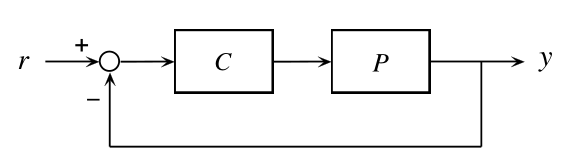
\includegraphics[width=0.3\linewidth]{./images/guadagno_anello_esempio_ben_connesso.png}
  \caption{Esempio di sistema ben connesso}
  \label{fig:guadagno_anello_esempio_ben_connesso}
\end{figure}


In questo caso il sistema è ben connesso se:
\begin{equation}
  \lim_{s \to \infty} 1 + C(s)P(s) \neq 0
\end{equation}



\begin{definition}[Stabilità asintotica interna]
  Il sistema retroazionato è asintoticamente ed internamente stabile quando
  tutte le funzioni di trasferimento fra gli ingresi e le uscite sono asintoticamente 
  stabili.

  Il sistema retrazionato è stabile asintoticamente ed internamente se e solo se:
  \begin{enumerate}
    \item Le radici dell'equazione $1 + C(s)P(s) = 0$ sono tutte a parte reale negativa
    \item le eventuali cancellazioni polo-zero fra $C(s)$ e $P(s)$ avvengono in $\mathbb{C_-}$
  \end{enumerate}
\end{definition}


La funzione di sensitività è:
\begin{equation}
  S(s) = \frac{1}{1 + C(s)P(s)}
\end{equation}

Mentre la sensitività complementare è:
\begin{equation}
  T(s) = \frac{C(s)P(s)}{1 + C(s)P(s)} = 1 - S
\end{equation}


\subsection{Controllori di struttura prefissata}
\begin{definition}
  I controllori di struttura prefissata sono definiti mediante particolari 
  parametrizzazioni della funzione di trasferimento del controllore.
\end{definition}

Si identificano due classi di controllori:
\begin{enumerate}
  \item Reti correttrici(correggono il comportamento dinamico della retrazione)
  \item regolatori standard(azioni proporzionali, derivative ed integrative)
\end{enumerate}

\newpage
\subsection{Le principali reti correttrici}
\begin{table}[h!]
  \centering
  \begin{tabular}{|c|c|c|}
    \hline
    Rete & Funzione & Grafico \\
    \hline
    \hline
    Integratrice & $C(s) = \frac{1}{1 + \tau s}, \tau > 0$ & 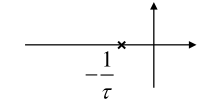
\includegraphics[width=0.15\linewidth]{./images/rete_integratrice.png} \\
    \hline
    Derivatrice & $C(s) = \frac{\tau s}{1 + \tau s}, \tau > 0$ & 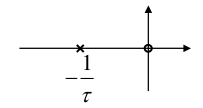
\includegraphics[width=0.15\linewidth]{./images/rete_derivatrice.png} \\
    \hline
    Ritardatrice & $C(s) = \frac{1 + \alpha \tau s}{1 + \tau s}, \tau > 0, \alpha \in (0, 1)$ & 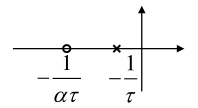
\includegraphics[width=0.15\linewidth]{./images/rete_ritardatrice.png} \\
    \hline
    Anticipatrice & $C(s) = \frac{1 + \tau s}{1 + \alpha \tau s}, \tau > 0, \alpha \in (0, 1)$ & 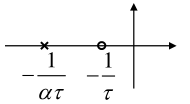
\includegraphics[width=0.15\linewidth]{./images/rete_anticipatrice.png} \\
    \hline
    Ritardo e anticipo & $C(s) = \frac{1 + 2 \delta' \frac{s}{\omega_n} + \frac{s^2}{\omega^2_n}}{1 + 2 \delta \frac{s}{\omega_n} + \frac{s^2}{\omega^2_n}}, \omega_n > 0, \delta > \delta' \geq 1$ & 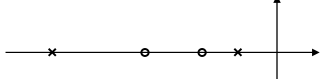
\includegraphics[width=0.15\linewidth]{./images/rete_ritardo_anticipo.png} \\
    \hline
    Rete a T ponticellato & $C(s) = \frac{1 + 2 \delta' \frac{s}{\omega_n} + \frac{s^2}{\omega^2_n}}{1 + 2 \delta \frac{s}{\omega_n} + \frac{s^2}{\omega^2_n}}, \omega_n > 0, \delta > 1,  \delta > \delta' > 0$ & 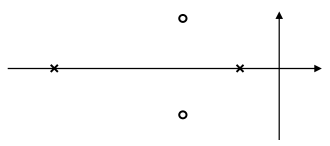
\includegraphics[width=0.15\linewidth]{./images/rete_t_ponticellato.png} \\
    \hline
  \end{tabular}
\end{table}

\subsection{I regolatori standard}

\begin{table}[h!]
  \centering
  \begin{tabular}{||c | c||}
  \hline
  Regolatore & Funzione \\
  \hline
  \hline
  Proporzionale (\textbf{P}) & $C(s) = K$ \\
  Integrale (\textbf{I})& $C(s) = \frac{K}{T_i s}$ \\
  Proporzionale-Integrativo (\textbf{PI}) & $C(s) = K(1 + \frac{1}{T_i s})$ \\
  Proporzionale-Derivativo (\textbf{PD}) & $C(s) = K(1 + T_d s)$ \\
  Proporzionale-Integrativo-Derivativo (\textbf{PID}) & $C(s) = K(1 + \frac{1}{T_i s} + T_d s)$ \\
  \hline
  \end{tabular}
\end{table}
  
\newpage
\subsection{La rete ritardatrice}
La rete ritardatrice è definita da:
\begin{equation}
  C_r = \frac{1 + \alpha \tau s}{1 + \tau s}
  \label{eq:rete_ritardatrice}
\end{equation}

Il diagramm di bode:
\begin{figure}[h!]
  \centering
  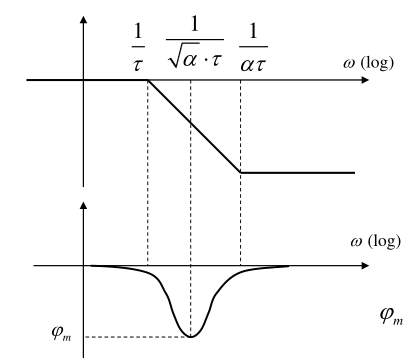
\includegraphics[width=0.3\linewidth]{./images/rete_ritardatrice_bode.png}
  \caption{Diagramma di bode della rete ritardatrice}
  \label{fig:rete_ritardatrice_bode}
\end{figure}

\begin{equation}
 \varphi_m = -\arcsin \frac{1 - \alpha}{1 + \alpha} 
\end{equation}
\begin{equation}
 \varphi_m = \arg C_r(j\omega_n)
\end{equation}
Dove:
\begin{equation}
  \omega_n := \frac{1}{\sqrt{\alpha} \cdot \tau}
\end{equation}


Questo controllo si utilizza quando il diagramma di nyquist super il punto critico -1
e si vuole far avvicinare il grafico verso lo 0.

\subsection{La rete anticipatrice}
Definita come:
\begin{equation}
  C_r(s) = \frac{1 + \tau s}{1 + \alpha \tau s}
  \label{eq:rete_anticipatrice}
\end{equation}

\begin{figure}[h!]
  \centering
  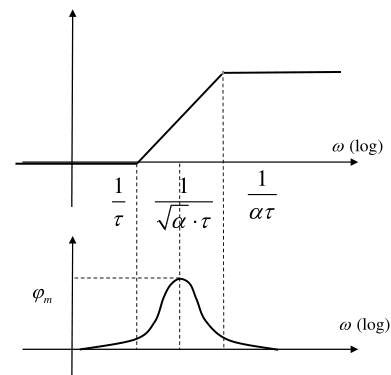
\includegraphics[width=0.3\linewidth]{./images/rete_anticipatrice_bode.png}
  \caption{Diagramma di bode della rete anticipatrice}
  \label{fig:rete_anticipatrice_bode}
\end{figure}

I vantaggi della rete anticipatrice sono:
\begin{itemize}
  \item Mantiene le prestazioni statiche come la rete ritardatrice
  \item Stabilizzza e allarga la banda
\end{itemize}

Gli svantaddi della rete anticipatrice sono inerenti all'introduzione di
rumore($\alpha$ non può essere troppo piccolo).

\subsection{Sintesi della rete anticipatrice per cancellazione polo-zero}
Si sceglie quale zero della rete il polo reale negativo di $P(s)$ più vicino
all’asse immaginario determinando così nella funzione di trasferimento di
catena diretta una cancellazione polo-zero (ammissibile).
